

\tikzset{every picture/.style={line width=0.75pt}} %set default line width to 0.75pt

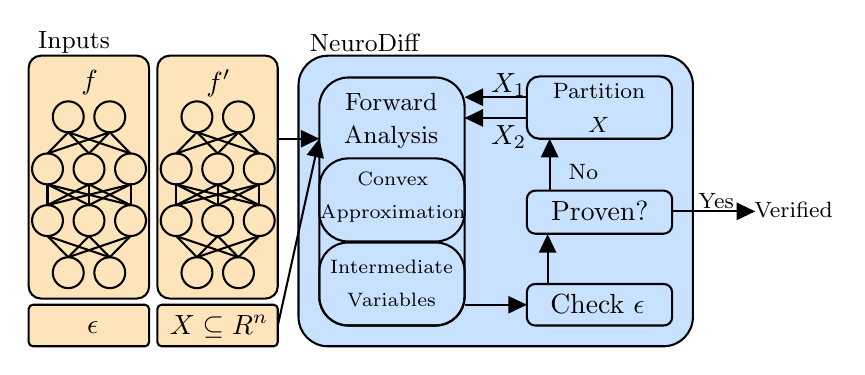
\begin{tikzpicture}[x=0.75pt,y=0.75pt,yscale=-1,xscale=1]
%uncomment if require: \path (0,300); %set diagram left start at 0, and has height of 300

%Rounded Rect [id:dp4236892252286144]
\draw  [fill={rgb, 255:red, 252; green, 202; blue, 120 }  ,fill opacity=0.5 ] (112,65.85) .. controls (112,62.62) and (114.62,60) .. (117.85,60) -- (164.15,60) .. controls (167.38,60) and (170,62.62) .. (170,65.85) -- (170,171.15) .. controls (170,174.38) and (167.38,177) .. (164.15,177) -- (117.85,177) .. controls (114.62,177) and (112,174.38) .. (112,171.15) -- cycle ;
%Shape: Circle [id:dp7068459723221313]
\draw   (123.61,89.44) .. controls (123.61,85.33) and (126.94,82) .. (131.06,82) .. controls (135.17,82) and (138.5,85.33) .. (138.5,89.44) .. controls (138.5,93.56) and (135.17,96.89) .. (131.06,96.89) .. controls (126.94,96.89) and (123.61,93.56) .. (123.61,89.44) -- cycle ;
%Shape: Circle [id:dp10436586105910262]
\draw   (143.61,89.44) .. controls (143.61,85.33) and (146.94,82) .. (151.06,82) .. controls (155.17,82) and (158.5,85.33) .. (158.5,89.44) .. controls (158.5,93.56) and (155.17,96.89) .. (151.06,96.89) .. controls (146.94,96.89) and (143.61,93.56) .. (143.61,89.44) -- cycle ;
%Shape: Circle [id:dp04586875504356169]
\draw   (113.61,114.56) .. controls (113.61,110.44) and (116.94,107.11) .. (121.06,107.11) .. controls (125.17,107.11) and (128.5,110.44) .. (128.5,114.56) .. controls (128.5,118.67) and (125.17,122) .. (121.06,122) .. controls (116.94,122) and (113.61,118.67) .. (113.61,114.56) -- cycle ;
%Shape: Circle [id:dp23529117657421317]
\draw   (133.61,114.56) .. controls (133.61,110.44) and (136.94,107.11) .. (141.06,107.11) .. controls (145.17,107.11) and (148.5,110.44) .. (148.5,114.56) .. controls (148.5,118.67) and (145.17,122) .. (141.06,122) .. controls (136.94,122) and (133.61,118.67) .. (133.61,114.56) -- cycle ;
%Shape: Circle [id:dp18975621582850755]
\draw   (153.61,114.56) .. controls (153.61,110.44) and (156.94,107.11) .. (161.06,107.11) .. controls (165.17,107.11) and (168.5,110.44) .. (168.5,114.56) .. controls (168.5,118.67) and (165.17,122) .. (161.06,122) .. controls (156.94,122) and (153.61,118.67) .. (153.61,114.56) -- cycle ;
%Straight Lines [id:da39358625060202257]
\draw    (131.06,96.89) -- (121.06,107.11) ;
%Straight Lines [id:da7050149301027024]
\draw    (131.06,96.89) -- (141.06,107.11) ;
%Straight Lines [id:da078846190833607]
\draw    (131.06,96.89) -- (161.06,107.11) ;
%Straight Lines [id:da2611151157782621]
\draw    (151.06,96.89) -- (161.06,107.11) ;
%Straight Lines [id:da854791249594143]
\draw    (151.06,96.89) -- (141.06,107.11) ;
%Straight Lines [id:da003907601781767633]
\draw    (151.06,96.89) -- (121.06,107.11) ;
%Shape: Circle [id:dp5156337693032028]
\draw   (158.5,164.56) .. controls (158.5,168.67) and (155.17,172) .. (151.06,172) .. controls (146.94,172) and (143.61,168.67) .. (143.61,164.56) .. controls (143.61,160.44) and (146.94,157.11) .. (151.06,157.11) .. controls (155.17,157.11) and (158.5,160.44) .. (158.5,164.56) -- cycle ;
%Shape: Circle [id:dp06607101355690326]
\draw   (138.5,164.56) .. controls (138.5,168.67) and (135.17,172) .. (131.06,172) .. controls (126.94,172) and (123.61,168.67) .. (123.61,164.56) .. controls (123.61,160.44) and (126.94,157.11) .. (131.06,157.11) .. controls (135.17,157.11) and (138.5,160.44) .. (138.5,164.56) -- cycle ;
%Shape: Circle [id:dp10601416223357618]
\draw   (168.5,139.44) .. controls (168.5,143.56) and (165.17,146.89) .. (161.06,146.89) .. controls (156.94,146.89) and (153.61,143.56) .. (153.61,139.44) .. controls (153.61,135.33) and (156.94,132) .. (161.06,132) .. controls (165.17,132) and (168.5,135.33) .. (168.5,139.44) -- cycle ;
%Shape: Circle [id:dp25720293065397004]
\draw   (148.5,139.44) .. controls (148.5,143.56) and (145.17,146.89) .. (141.06,146.89) .. controls (136.94,146.89) and (133.61,143.56) .. (133.61,139.44) .. controls (133.61,135.33) and (136.94,132) .. (141.06,132) .. controls (145.17,132) and (148.5,135.33) .. (148.5,139.44) -- cycle ;
%Shape: Circle [id:dp4093542080553124]
\draw   (128.5,139.44) .. controls (128.5,143.56) and (125.17,146.89) .. (121.06,146.89) .. controls (116.94,146.89) and (113.61,143.56) .. (113.61,139.44) .. controls (113.61,135.33) and (116.94,132) .. (121.06,132) .. controls (125.17,132) and (128.5,135.33) .. (128.5,139.44) -- cycle ;
%Straight Lines [id:da8322313642706787]
\draw    (151.06,157.11) -- (161.06,146.89) ;
%Straight Lines [id:da4076421006538775]
\draw    (151.06,157.11) -- (141.06,146.89) ;
%Straight Lines [id:da22036650281611347]
\draw    (151.06,157.11) -- (121.06,146.89) ;
%Straight Lines [id:da5955438584611725]
\draw    (131.06,157.11) -- (121.06,146.89) ;
%Straight Lines [id:da6153976114126399]
\draw    (131.06,157.11) -- (141.06,146.89) ;
%Straight Lines [id:da9953813996835473]
\draw    (131.06,157.11) -- (161.06,146.89) ;

%Straight Lines [id:da23986906826746157]
\draw    (121.06,122) -- (141.06,132) ;
%Straight Lines [id:da2936393327105673]
\draw    (121.06,122) -- (161.06,132) ;
%Straight Lines [id:da5774592223000948]
\draw    (141.06,122) -- (121.06,132) ;
%Straight Lines [id:da027247136169882613]
\draw    (141.06,122) -- (141.06,132) ;
%Straight Lines [id:da2078286476738037]
\draw    (141.06,122) -- (161.06,132) ;
%Straight Lines [id:da07067307391973043]
\draw    (161.06,122) -- (161.06,132) ;
%Straight Lines [id:da5480660909270823]
\draw    (161.06,122) -- (141.06,132) ;
%Straight Lines [id:da6293253437621619]
\draw    (161.06,122) -- (121.06,132) ;
%Straight Lines [id:da7407175241217754]
\draw    (121.06,122) -- (121.06,132) ;

%Rounded Rect [id:dp2355420157466821]
\draw  [fill={rgb, 255:red, 252; green, 202; blue, 120 }  ,fill opacity=0.5 ] (50,182.02) .. controls (50,180.9) and (50.9,180) .. (52.02,180) -- (105.98,180) .. controls (107.1,180) and (108,180.9) .. (108,182.02) -- (108,197.98) .. controls (108,199.1) and (107.1,200) .. (105.98,200) -- (52.02,200) .. controls (50.9,200) and (50,199.1) .. (50,197.98) -- cycle ;
%Rounded Rect [id:dp39333818742980176]
\draw  [fill={rgb, 255:red, 144; green, 195; blue, 255 }  ,fill opacity=0.5 ] (180,74.13) .. controls (180,66.33) and (186.33,60) .. (194.13,60) -- (355.87,60) .. controls (363.67,60) and (370,66.33) .. (370,74.13) -- (370,185.87) .. controls (370,193.67) and (363.67,200) .. (355.87,200) -- (194.13,200) .. controls (186.33,200) and (180,193.67) .. (180,185.87) -- cycle ;
%Rounded Rect [id:dp15859389295109172]
\draw   (246,70.5) .. controls (253.73,70.5) and (260,76.77) .. (260,84.5) -- (260,176) .. controls (260,183.73) and (253.73,190) .. (246,190) -- (204,190) .. controls (196.27,190) and (190,183.73) .. (190,176) -- (190,84.5) .. controls (190,76.77) and (196.27,70.5) .. (204,70.5) -- cycle ;
%Straight Lines [id:da09167228503135971]
\draw    (170,100) -- (187,100) ;
\draw [shift={(190,100)}, rotate = 180] [fill={rgb, 255:red, 0; green, 0; blue, 0 }  ][line width=0.08]  [draw opacity=0] (8.93,-4.29) -- (0,0) -- (8.93,4.29) -- cycle    ;
%Straight Lines [id:da15082942023264767]
\draw    (170,190) -- (189.35,102.93) ;
\draw [shift={(190,100)}, rotate = 462.53] [fill={rgb, 255:red, 0; green, 0; blue, 0 }  ][line width=0.08]  [draw opacity=0] (8.93,-4.29) -- (0,0) -- (8.93,4.29) -- cycle    ;
%Rounded Rect [id:dp19836331083326175]
\draw  [fill={rgb, 255:red, 252; green, 202; blue, 120 }  ,fill opacity=0.5 ] (112,182.02) .. controls (112,180.9) and (112.9,180) .. (114.02,180) -- (167.98,180) .. controls (169.1,180) and (170,180.9) .. (170,182.02) -- (170,197.98) .. controls (170,199.1) and (169.1,200) .. (167.98,200) -- (114.02,200) .. controls (112.9,200) and (112,199.1) .. (112,197.98) -- cycle ;
%Rounded Rect [id:dp3414447171885684]
\draw   (190,163.86) .. controls (190,156.2) and (196.2,150) .. (203.86,150) -- (246.14,150) .. controls (253.8,150) and (260,156.2) .. (260,163.86) -- (260,176.14) .. controls (260,183.8) and (253.8,190) .. (246.14,190) -- (203.86,190) .. controls (196.2,190) and (190,183.8) .. (190,176.14) -- cycle ;
%Rounded Rect [id:dp7331605414728447]
\draw   (190,123.36) .. controls (190,115.7) and (196.2,109.5) .. (203.86,109.5) -- (246.14,109.5) .. controls (253.8,109.5) and (260,115.7) .. (260,123.36) -- (260,135.64) .. controls (260,143.3) and (253.8,149.5) .. (246.14,149.5) -- (203.86,149.5) .. controls (196.2,149.5) and (190,143.3) .. (190,135.64) -- cycle ;
%Rounded Rect [id:dp724286819012004]
\draw   (356,170) .. controls (358.21,170) and (360,171.79) .. (360,174) -- (360,186) .. controls (360,188.21) and (358.21,190) .. (356,190) -- (294,190) .. controls (291.79,190) and (290,188.21) .. (290,186) -- (290,174) .. controls (290,171.79) and (291.79,170) .. (294,170) -- cycle ;
%Rounded Rect [id:dp8526981920637079]
\draw   (355.84,125) .. controls (358.14,125) and (360,126.86) .. (360,129.16) -- (360,141.62) .. controls (360,143.92) and (358.14,145.78) .. (355.84,145.78) -- (294.16,145.78) .. controls (291.86,145.78) and (290,143.92) .. (290,141.62) -- (290,129.16) .. controls (290,126.86) and (291.86,125) .. (294.16,125) -- cycle ;
%Rounded Rect [id:dp6803009958438129]
\draw   (354,70) .. controls (357.31,70) and (360,72.69) .. (360,76) -- (360,94) .. controls (360,97.31) and (357.31,100) .. (354,100) -- (296,100) .. controls (292.69,100) and (290,97.31) .. (290,94) -- (290,76) .. controls (290,72.69) and (292.69,70) .. (296,70) -- cycle ;
%Straight Lines [id:da323377208231176]
\draw    (300,170) -- (300,149) ;
\draw [shift={(300,146)}, rotate = 450] [fill={rgb, 255:red, 0; green, 0; blue, 0 }  ][line width=0.08]  [draw opacity=0] (8.93,-4.29) -- (0,0) -- (8.93,4.29) -- cycle    ;
%Straight Lines [id:da9479303756560082]
\draw    (301,125) -- (301,103) ;
\draw [shift={(301,100)}, rotate = 450] [fill={rgb, 255:red, 0; green, 0; blue, 0 }  ][line width=0.08]  [draw opacity=0] (8.93,-4.29) -- (0,0) -- (8.93,4.29) -- cycle    ;
%Straight Lines [id:da32236695764284484]
\draw    (260,180) -- (287,180) ;
\draw [shift={(290,180)}, rotate = 180] [fill={rgb, 255:red, 0; green, 0; blue, 0 }  ][line width=0.08]  [draw opacity=0] (8.93,-4.29) -- (0,0) -- (8.93,4.29) -- cycle    ;
%Straight Lines [id:da551116351892766]
\draw    (360,135) -- (397,135) ;
\draw [shift={(400,135)}, rotate = 180] [fill={rgb, 255:red, 0; green, 0; blue, 0 }  ][line width=0.08]  [draw opacity=0] (8.93,-4.29) -- (0,0) -- (8.93,4.29) -- cycle    ;
%Rounded Rect [id:dp9869780674255966]
\draw  [fill={rgb, 255:red, 252; green, 202; blue, 120 }  ,fill opacity=0.5 ] (50,65.85) .. controls (50,62.62) and (52.62,60) .. (55.85,60) -- (102.15,60) .. controls (105.38,60) and (108,62.62) .. (108,65.85) -- (108,171.15) .. controls (108,174.38) and (105.38,177) .. (102.15,177) -- (55.85,177) .. controls (52.62,177) and (50,174.38) .. (50,171.15) -- cycle ;
%Shape: Circle [id:dp8539692235458093]
\draw   (61.61,89.44) .. controls (61.61,85.33) and (64.94,82) .. (69.06,82) .. controls (73.17,82) and (76.5,85.33) .. (76.5,89.44) .. controls (76.5,93.56) and (73.17,96.89) .. (69.06,96.89) .. controls (64.94,96.89) and (61.61,93.56) .. (61.61,89.44) -- cycle ;
%Shape: Circle [id:dp1487342990764624]
\draw   (81.61,89.44) .. controls (81.61,85.33) and (84.94,82) .. (89.06,82) .. controls (93.17,82) and (96.5,85.33) .. (96.5,89.44) .. controls (96.5,93.56) and (93.17,96.89) .. (89.06,96.89) .. controls (84.94,96.89) and (81.61,93.56) .. (81.61,89.44) -- cycle ;
%Shape: Circle [id:dp35573619874650775]
\draw   (51.61,114.56) .. controls (51.61,110.44) and (54.94,107.11) .. (59.06,107.11) .. controls (63.17,107.11) and (66.5,110.44) .. (66.5,114.56) .. controls (66.5,118.67) and (63.17,122) .. (59.06,122) .. controls (54.94,122) and (51.61,118.67) .. (51.61,114.56) -- cycle ;
%Shape: Circle [id:dp43998418948198004]
\draw   (71.61,114.56) .. controls (71.61,110.44) and (74.94,107.11) .. (79.06,107.11) .. controls (83.17,107.11) and (86.5,110.44) .. (86.5,114.56) .. controls (86.5,118.67) and (83.17,122) .. (79.06,122) .. controls (74.94,122) and (71.61,118.67) .. (71.61,114.56) -- cycle ;
%Shape: Circle [id:dp11364870191253851]
\draw   (91.61,114.56) .. controls (91.61,110.44) and (94.94,107.11) .. (99.06,107.11) .. controls (103.17,107.11) and (106.5,110.44) .. (106.5,114.56) .. controls (106.5,118.67) and (103.17,122) .. (99.06,122) .. controls (94.94,122) and (91.61,118.67) .. (91.61,114.56) -- cycle ;
%Straight Lines [id:da5311768222051036]
\draw    (69.06,96.89) -- (59.06,107.11) ;
%Straight Lines [id:da8245862905976873]
\draw    (69.06,96.89) -- (79.06,107.11) ;
%Straight Lines [id:da9037048113348528]
\draw    (69.06,96.89) -- (99.06,107.11) ;
%Straight Lines [id:da6775367181725077]
\draw    (89.06,96.89) -- (99.06,107.11) ;
%Straight Lines [id:da20764974600729147]
\draw    (89.06,96.89) -- (79.06,107.11) ;
%Straight Lines [id:da4787036285423938]
\draw    (89.06,96.89) -- (59.06,107.11) ;
%Shape: Circle [id:dp6787178527201608]
\draw   (96.5,164.56) .. controls (96.5,168.67) and (93.17,172) .. (89.06,172) .. controls (84.94,172) and (81.61,168.67) .. (81.61,164.56) .. controls (81.61,160.44) and (84.94,157.11) .. (89.06,157.11) .. controls (93.17,157.11) and (96.5,160.44) .. (96.5,164.56) -- cycle ;
%Shape: Circle [id:dp8189142658483558]
\draw   (76.5,164.56) .. controls (76.5,168.67) and (73.17,172) .. (69.06,172) .. controls (64.94,172) and (61.61,168.67) .. (61.61,164.56) .. controls (61.61,160.44) and (64.94,157.11) .. (69.06,157.11) .. controls (73.17,157.11) and (76.5,160.44) .. (76.5,164.56) -- cycle ;
%Shape: Circle [id:dp21275076334366427]
\draw   (106.5,139.44) .. controls (106.5,143.56) and (103.17,146.89) .. (99.06,146.89) .. controls (94.94,146.89) and (91.61,143.56) .. (91.61,139.44) .. controls (91.61,135.33) and (94.94,132) .. (99.06,132) .. controls (103.17,132) and (106.5,135.33) .. (106.5,139.44) -- cycle ;
%Shape: Circle [id:dp1824568474340943]
\draw   (86.5,139.44) .. controls (86.5,143.56) and (83.17,146.89) .. (79.06,146.89) .. controls (74.94,146.89) and (71.61,143.56) .. (71.61,139.44) .. controls (71.61,135.33) and (74.94,132) .. (79.06,132) .. controls (83.17,132) and (86.5,135.33) .. (86.5,139.44) -- cycle ;
%Shape: Circle [id:dp825767248504503]
\draw   (66.5,139.44) .. controls (66.5,143.56) and (63.17,146.89) .. (59.06,146.89) .. controls (54.94,146.89) and (51.61,143.56) .. (51.61,139.44) .. controls (51.61,135.33) and (54.94,132) .. (59.06,132) .. controls (63.17,132) and (66.5,135.33) .. (66.5,139.44) -- cycle ;
%Straight Lines [id:da6766885451674735]
\draw    (89.06,157.11) -- (99.06,146.89) ;
%Straight Lines [id:da08122409377631135]
\draw    (89.06,157.11) -- (79.06,146.89) ;
%Straight Lines [id:da8441374241505181]
\draw    (89.06,157.11) -- (59.06,146.89) ;
%Straight Lines [id:da7442737845395763]
\draw    (69.06,157.11) -- (59.06,146.89) ;
%Straight Lines [id:da9566636567575862]
\draw    (69.06,157.11) -- (79.06,146.89) ;
%Straight Lines [id:da19409192754236826]
\draw    (69.06,157.11) -- (99.06,146.89) ;

%Straight Lines [id:da39227385116907143]
\draw    (59.06,122) -- (79.06,132) ;
%Straight Lines [id:da16288130182449367]
\draw    (59.06,122) -- (99.06,132) ;
%Straight Lines [id:da19810001689574364]
\draw    (79.06,122) -- (59.06,132) ;
%Straight Lines [id:da24191813694330322]
\draw    (79.06,122) -- (79.06,132) ;
%Straight Lines [id:da1525732415062876]
\draw    (79.06,122) -- (99.06,132) ;
%Straight Lines [id:da22405676573237499]
\draw    (99.06,122) -- (99.06,132) ;
%Straight Lines [id:da9334192766546668]
\draw    (99.06,122) -- (79.06,132) ;
%Straight Lines [id:da3285219924463475]
\draw    (99.06,122) -- (59.06,132) ;
%Straight Lines [id:da28988712234136327]
\draw    (59.06,122) -- (59.06,132) ;

%Straight Lines [id:da08693151331707771]
\draw    (290,80) -- (263,80) ;
\draw [shift={(260,80)}, rotate = 360] [fill={rgb, 255:red, 0; green, 0; blue, 0 }  ][line width=0.08]  [draw opacity=0] (8.93,-4.29) -- (0,0) -- (8.93,4.29) -- cycle    ;
%Straight Lines [id:da3246311983059058]
\draw    (290,90) -- (263,90) ;
\draw [shift={(260,90)}, rotate = 360] [fill={rgb, 255:red, 0; green, 0; blue, 0 }  ][line width=0.08]  [draw opacity=0] (8.93,-4.29) -- (0,0) -- (8.93,4.29) -- cycle    ;

% Text Node
\draw (53,47) node [anchor=north west][inner sep=0.75pt]   [align=left] {\small
Inputs};
% Text Node
\draw (184,48) node [anchor=north west][inner sep=0.75pt]   [align=left] {\small
NeuroDiff};
% Text Node
\draw (196,76.5) node [anchor=north west][inner sep=0.75pt]   [align=left] {\begin{minipage}[lt]{40.70935600000001pt}\setlength\topsep{0pt}
	\begin{center}
	{\small Forward}\\{\small Analysis}
	\end{center}

	\end{minipage}};
% Text Node
\draw (183,114.5) node [anchor=north west][inner sep=0.75pt]   [align=left] {\begin{minipage}[lt]{61.370000000000005pt}\setlength\topsep{0pt}
	\begin{center}
	{\scriptsize Convex}\\{\scriptsize Approximation}
	\end{center}

	\end{minipage}};
% Text Node
\draw (187.5,157) node [anchor=north west][inner sep=0.75pt]   [align=left] {\begin{minipage}[lt]{53.720000000000006pt}\setlength\topsep{0pt}
	\begin{center}
	{\scriptsize Intermediate}\\{\scriptsize Variables}
	\end{center}

	\end{minipage}};
% Text Node
\draw (296,173.5) node [anchor=north west][inner sep=0.75pt]   [align=left] {\begin{minipage}[lt]{39.848000000000006pt}\setlength\topsep{0pt}
	\begin{center}
	Check $\displaystyle \epsilon $
	\end{center}

	\end{minipage}};
% Text Node
\draw (369,125) node [anchor=north west][inner sep=0.75pt]  [font=\footnotesize] [align=left] {\begin{minipage}[lt]{16.025356000000002pt}\setlength\topsep{0pt}
	\begin{center}
	Yes
	\end{center}

	\end{minipage}};
% Text Node
\draw (397,129) node [anchor=north west][inner sep=0.75pt]  [font=\footnotesize] [align=left] {\begin{minipage}[lt]{29.931356pt}\setlength\topsep{0pt}
	\begin{center}
	Verified
	\end{center}

	\end{minipage}};
% Text Node
\draw (296.5,72) node [anchor=north west][inner sep=0.75pt]   [align=left] {\begin{minipage}[lt]{40.154pt}\setlength\topsep{0pt}
	\begin{center}
	{\footnotesize Partition $\displaystyle X$}
	\end{center}

	\end{minipage}};
% Text Node
\draw (307,111) node [anchor=north west][inner sep=0.75pt]  [font=\footnotesize] [align=left] {\begin{minipage}[lt]{13.146644000000002pt}\setlength\topsep{0pt}
	\begin{center}
	No
	\end{center}

	\end{minipage}};
% Text Node
\draw (57.56,65.5) node [anchor=north west][inner sep=0.75pt]   [align=left] {\begin{minipage}[lt]{30.498000000000005pt}\setlength\topsep{0pt}
	\begin{center}
	$ f $
	\end{center}

	\end{minipage}};
% Text Node
\draw (119.56,65.5) node [anchor=north west][inner sep=0.75pt]   [align=left] {\begin{minipage}[lt]{30.498000000000005pt}\setlength\topsep{0pt}
	\begin{center}
	$ f' $
	\end{center}

	\end{minipage}};
% Text Node
\draw (113.06,183.5) node [anchor=north west][inner sep=0.75pt]   [align=left] {\begin{minipage}[lt]{40.63pt}\setlength\topsep{0pt}
	\begin{center}
	$\displaystyle X\subseteq \mathbb{R}^{n}$
	\end{center}

	\end{minipage}};
% Text Node
\draw (73.56,186.5) node [anchor=north west][inner sep=0.75pt]   [align=left] {\begin{minipage}[lt]{8.67pt}\setlength\topsep{0pt}
	\begin{center}
	$\displaystyle \epsilon $
	\end{center}

	\end{minipage}};
% Text Node
\draw (269,67) node [anchor=north west][inner sep=0.75pt]   [align=left] {\begin{minipage}[lt]{16.127356000000002pt}\setlength\topsep{0pt}
	\begin{center}
	$\displaystyle X_{1}$
	\end{center}

	\end{minipage}};
% Text Node
\draw (269,92) node [anchor=north west][inner sep=0.75pt]   [align=left] {\begin{minipage}[lt]{16.127356000000002pt}\setlength\topsep{0pt}
	\begin{center}
	$\displaystyle X_{2}$
	\end{center}

	\end{minipage}};
% Text Node
\draw (296.5,128.83) node [anchor=north west][inner sep=0.75pt]   [align=left] {\begin{minipage}[lt]{40.732pt}\setlength\topsep{0pt}
	\begin{center}
	Proven?
	\end{center}

	\end{minipage}};


\end{tikzpicture}
